% \documentclass{book}

\documentclass[12pt]{article}
\usepackage[pdfborder={0 0 0.5 [3 2]}]{hyperref}%
\usepackage[left=1in,right=1in,top=1in,bottom=1in]{geometry}%
\usepackage[shortalphabetic]{amsrefs}%
\usepackage{amsmath}
\usepackage{enumerate}
\usepackage{enumitem}
\usepackage{amssymb}                
\usepackage{amsmath}                
\usepackage{amsfonts}
\usepackage{amsthm}
\usepackage{bbm}
\usepackage[table,xcdraw]{xcolor}
\usepackage{tikz}
\usepackage{float}
\usepackage{booktabs}
\usepackage{svg}
\usepackage{mathtools}
\usepackage{cool}
\usepackage{url}
\usepackage{graphicx,epsfig}
\usepackage{framed}
\usepackage{hyperref}  

\usetikzlibrary{automata,arrows,positioning,calc}
\DeclarePairedDelimiter\abs{\lvert}{\rvert}%
\DeclarePairedDelimiter\norm{\lVert}{\rVert}%
\DeclarePairedDelimiter\ceil{\lceil}{\rceil}
\DeclarePairedDelimiter\floor{\lfloor}{\rfloor}

\makeatletter
\renewcommand*\env@matrix[1][*\c@MaxMatrixCols c]{%
  \hskip -\arraycolsep
  \let\@ifnextchar\new@ifnextchar
  \array{#1}}
\makeatother

\newtheorem{theorem}{Theorem}[section]
\newtheorem{corollary}{Corollary}[theorem]
\newtheorem{proposition}[theorem]{Proposition}
\newtheorem{lemma}[theorem]{Lemma}

\theoremstyle{definition}
\newtheorem{definition}[theorem]{Definition}
\newtheorem{exercise}{Exercise}%
\newtheorem{problem}[exercise]{Problem}%
\newtheorem*{example}{Example}

\theoremstyle{remark}
\newtheorem*{question}{Question}
\newtheorem*{observation}{Observation}
\newtheorem*{remark}{Remark}

\graphicspath{ {images/} }

\setlength{\parindent}{0cm}
\renewcommand{\vec}[1]{\ensuremath{\mathbf{#1}}}

\def\noi{\noindent}
\def\T{{\mathbb T}}
\def\R{{\mathbb R}}
\def\N{{\mathbb N}}
\def\C{{\mathbb C}}
\def\Z{{\mathbb Z}}
\def\P{{\mathbb P}}
\def\E{{\mathbb E}}
\def\Q{\mathbb{Q}}
\def\ind{{\mathbb I}}

\def\cale{{\mathcal E}}
\def\cals{{\mathcal S}}
\def\calc{{\mathcal C}}
\def\caln{{\mathcal N}}
\def\calb{{\mathcal B}}
\def\calg{{\cal G}}

\def\ds{\displaystyle}
\def\ra{\rightarrow}
\newcommand{\conv}{\mbox{\rm conv}}
\newcommand{\spaan}{\mbox{\rm span}}
\newcommand{\deet}{\mbox{\rm det}}
\newcommand{\aff}{\mbox{\rm aff}}
\newcommand{\cl}{\mbox{\rm cl}}
\newcommand{\dimm}{\mbox{\rm dim}}
\newcommand{\sm}{\setminus}
\def\ci{\perp\!\!\!\perp}


\newcommand{\ink}{\rule{.5\baselineskip}{.55\baselineskip}}

\begin{document}

\section{Probability Essentials}
In general parlance, the term \emph{probability} is used as a measure of a person's belief in the occurrence of an event. This is the \emph{subjective} notion of probability. Take a sentence such as, ``There is a 60\% probability of rain tomorrow''. Where did this come from? A professional meteorologist has used a sophisticated mathematical model to distill large amounts of atmospheric data down to a simple number indicating her belief that it is more likely to rain than to not rain tomorrow. We can intepret this number however we wish. We should be careful, however, to examine both our biases and those of the meterologist. Who does this meterologist work for? How reliable have their predictions been in the past? (We should be careful here since we might be more likely to recall rain when none was predicted than the other way around.) Are meterologists more likely to err on the side of predicting rain, since that way fewer people will be upset if they are wrong? We can use this number to make important life decisions such as whether or not to carry an umbrella. The downside of this is that it is in essence a subjective opinion, even if that opinion comes from an expert. In addition, for subjective probabilites to make sense, they have to be internally consistent. In this example, if we believe there is a 60\% chance of rain tomorrow, we must also believe that there is a 40\% chance of it not raining tomorrow.
\\

Let's look at a different example. What is the probability of rolling a 1 on a standard six-sided die? We can argue based on symmetry that since dice are cubical, there should be no reason for one face to be preferred over another. Thus this probability is 1/6. This is the \emph{classical} notion of probability. In this interpretation, we use symmetry arguments to divide our experiment (a single die roll, in this case) into elementary events which are equally probable (the six distint die rolls). We can compute the proability of any event using these elementary, equiprobably events. The limitation of this approach is that is requires a symmetry argument to be effective; thus it works for coin flips and die rolls, but not for more complicated scenarios.\\

We can look at the die roll experiment in another way. Imaging rolling a standard six-sided die repeatedly. The empirical probability of rolling a 1 is the ratio of the number of times a 1 is rolled to the total number of rolls. In general, we have:
\[
\text{empirical probability of a certain event} = \frac{ \text{number of times the event occurs }}{\text{total number of trials}}
\]
Intuitively, as we perform more and more dice rolls, the empirical probability of rolling a 1 should approach some mythical quantity which we call the \emph{true probability} of rolling a 1. This approach is the \emph{empirical}, or \emph{frequentist}, approach to probability. For a standard, six-sided die, it stands to reason that the empirical probabilty should approach the classical probabiliy of 1/6 as the number of rolls approaches infinity. This result is called the \emph{law of large numbers} and will be discussed later in the course. The empirical approach has a critical advantage over the classical approach in that we do not require symmetry to compute our probabilities. As an example of this, think of how you would determine the probability of rolling a 1 if someone handed you a loaded die. The empirical approach does, however, have its limits. Returing to the weather example, there is no way to think of the chance of rain tomorrow as the limit of a sequence of independent experiements. Unless we are in the movie Groundhog Day, tomorrow can only happen once!\\

For our purposes, we require a more rigorous, mathematical construction of probability. This is known as \emph{axiomatic probability} and will unify some of the aspects of the other approaches to probability. For this, we turn to the language of \emph{set theory}.

\subsection{Sample Spaces}
A \emph{set} is a collection of distinct objects. A \emph{sample space}, denoted $\cals$ is the set of all outcomes of a particular experiment. Here are some examples of sample spaces:
\begin{enumerate}
\item Single coin flip: $\cals = \{H, T\}$
\item Roll of one standard, six-sided die: $\cals = \{1, 2, 3, 4, 5, 6\}$
\item Roll of two standard, six-sided dice: Here we represent the sample spaces as ordered pairs.

\begin{figure}[H]
\centering
% \caption{My caption}
\label{twodice}
\begin{tabular}{llllllll}
           &                        &        &        & \multicolumn{2}{l}{second roll} &        &                             \\
           &                        & 1      & 2      & 3              & 4              & 5      & 6                           \\ \cline{3-8} 
           & \multicolumn{1}{l|}{1} & (1, 1) & (1, 2) & (1, 3)         & (1, 4)         & (1, 5) & \multicolumn{1}{l|}{(1, 6)} \\
           & \multicolumn{1}{l|}{2} & (2, 1) & (2, 2) & (2, 3)         & (2, 4)         & (2, 5) & \multicolumn{1}{l|}{(2, 6)} \\
first roll & \multicolumn{1}{l|}{3} & (3, 1) & (3, 2) & (3, 3)         & (3, 4)         & (3, 5) & \multicolumn{1}{l|}{(3, 6)} \\
           & \multicolumn{1}{l|}{4} & (4, 1) & (4, 2) & (4, 3)         & (4, 4)         & (4, 5) & \multicolumn{1}{l|}{(4, 6)} \\
           & \multicolumn{1}{l|}{5} & (5, 1) & (5, 2) & (5, 3)         & (5, 4)         & (5, 5) & \multicolumn{1}{l|}{(5, 6)} \\
           & \multicolumn{1}{l|}{6} & (6, 1) & (6, 2) & (6, 3)         & (6, 4)         & (6, 5) & \multicolumn{1}{l|}{(6, 6)} \\ \cline{3-8} 
\end{tabular}
\end{figure}

\item Number of free throw attempts it takes for me to make a single basket: $\cals = \{1, 2, 3, ...\}$. This set is often denoted $\N$ for the natural numbers (positive integers)
\item Number of minutes late my RIPTA bus arrives: $\cals = [0, \infty)$. 
\end{enumerate}
Note that the first three sample spaces contain only a finite number of elements (2, 6, and 36 elements, respectively). These are called \emph{finite sample spaces}. The fourth and fifth sample spaces both contain an infinite number of elements, but there is a fundamental difference between the two. The set $\N$ can be written out in its entirety in an infinitely long list; another way to think about this is that we can start at 1 and count up to any number in the set (as long as we have enough time!). A set with this property is called \emph{countable}. For the set $[0, \infty)$, it makes intuitive sense that we cannot do this, i.e. we cannot list all the elements and, say, ``count up to $\pi$''. A proof of this fact is left for another course. Such an infinite set is called \emph{uncountable}\footnote{An uncountable set is a ``larger infinity'' than a countable set, which leads to the concept of ``sizes of infinity''. John Green alludes to this in his novel \emph{The Fault in Our Stars}, but unforunately gets the math wrong. If you find this interesting, I recommend the Vi Hart video \url{https://www.youtube.com/watch?v=23I5GS4JiDg}}. A sample space which is either finite or countable is called \emph{discrete}.\\

\subsection{Events and Subsets}
An \emph{event} is a subset of a sample space. Events are usually designated by capital letters, and we write the relationship ``$A$ is a subset of $\cals$'' by $A \subset \cals$. For two events $A$ and $B$, $A \subset B$ if every element in $A$ is also contained in $B$. The \emph{empty set}, denoted $\emptyset$, is the set containing no elements, and it is a subset of every set.
\\

Let us consider the sample space $\cals = \{1, 2, 3, 4, 5, 6\}$, representing the roll of a single die. The following are examples of events:
\begin{enumerate}
\item $A = \{2, 4, 6\}$, the event that an even number is rolled
\item $B = \{1, 2, 3\}$, the event that the roll is less than or equal to 3
\item $C = \{1\}$, the event that a 1 is rolled
\end{enumerate}
The event $C$ consists of a single element in the sample space. Such an event is called a \emph{simple event} and cannot be decomposed. The events $A$ and $B$ are each composed of three simple events.\\

Next, consider the sample space repesenting rolls of two dice. Let $E$ be the event that the sum of the two dice is 7. We can represent this event graphically; in the figure below, the event $E$ consists of the squares which are highlighted in yellow.

% Please add the following required packages to your document preamble:
% \usepackage[table,xcdraw]{xcolor}
% If you use beamer only pass "xcolor=table" option, i.e. \documentclass[xcolor=table]{beamer}
\begin{figure}[H]
\centering
% \caption{My caption}
\label{two-dice-sum-seven}
\begin{tabular}{llllllll}
           &                        &                                                     &                                                     & \multicolumn{2}{l}{second roll}                                                                           &                                                     &                                                     \\
           &                        & 1                                                   & 2                                                   & 3                                                   & 4                                                   & 5                                                   & 6                                                   \\ \cline{3-8} 
           & \multicolumn{1}{l|}{1} & (1, 1)                                              & (1, 2)                                              & (1, 3)                                              & (1, 4)                                              & \multicolumn{1}{l|}{(1, 5)}                         & \multicolumn{1}{l|}{\cellcolor[HTML]{F8FF00}(1, 6)} \\ \cline{7-8} 
           & \multicolumn{1}{l|}{2} & (2, 1)                                              & (2, 2)                                              & (2, 3)                                              & \multicolumn{1}{l|}{(2, 4)}                         & \multicolumn{1}{l|}{\cellcolor[HTML]{F8FF00}(2, 5)} & \multicolumn{1}{l|}{(2, 6)}                         \\ \cline{6-7}
first roll & \multicolumn{1}{l|}{3} & (3, 1)                                              & (3, 2)                                              & \multicolumn{1}{l|}{(3, 3)}                         & \multicolumn{1}{l|}{\cellcolor[HTML]{F8FF00}(3, 4)} & (3, 5)                                              & \multicolumn{1}{l|}{(3, 6)}                         \\ \cline{5-6}
           & \multicolumn{1}{l|}{4} & (4, 1)                                              & \multicolumn{1}{l|}{(4, 2)}                         & \multicolumn{1}{l|}{\cellcolor[HTML]{F8FF00}(4, 3)} & (4, 4)                                              & (4, 5)                                              & \multicolumn{1}{l|}{(4, 6)}                         \\ \cline{4-5}
           & \multicolumn{1}{l|}{5} & \multicolumn{1}{l|}{(5, 1)}                         & \multicolumn{1}{l|}{\cellcolor[HTML]{F8FF00}(5, 2)} & (5, 3)                                              & (5, 4)                                              & (5, 5)                                              & \multicolumn{1}{l|}{(5, 6)}                         \\ \cline{3-4}
           & \multicolumn{1}{l|}{6} & \multicolumn{1}{l|}{\cellcolor[HTML]{F8FF00}(6, 1)} & (6, 2)                                              & (6, 3)                                              & (6, 4)                                              & (6, 5)                                              & \multicolumn{1}{l|}{(6, 6)}                         \\ \cline{3-8} 
\end{tabular}
\end{figure}

\subsection{Basic Set Operations}

\begin{quotation}
``You have multiple core competencies with surprisingly minimal Venn. You can pivot from working on astrophysics problems, to teaching the young Arkers, to podcasting to folks on the ground, without skipping a beat!'' - Neal Stephenson, \emph{Seveneves}
\end{quotation}

Let $\cals$ be our sample space, the set of all elements under consideration. Consider two events $A$ and $B$ which are subsets of $\cals$. We have the following three basic set operations, which are handily illustrated using Venn diagrams.
\begin{enumerate}
\item The \emph{union} of $A$ and $B$, denoted $A \cup B$, is the set of all elements which are in $A$ or $B$ (or both). That is, the union is all elements that are in at least one of the two sets.
\begin{figure}[H]
\centering
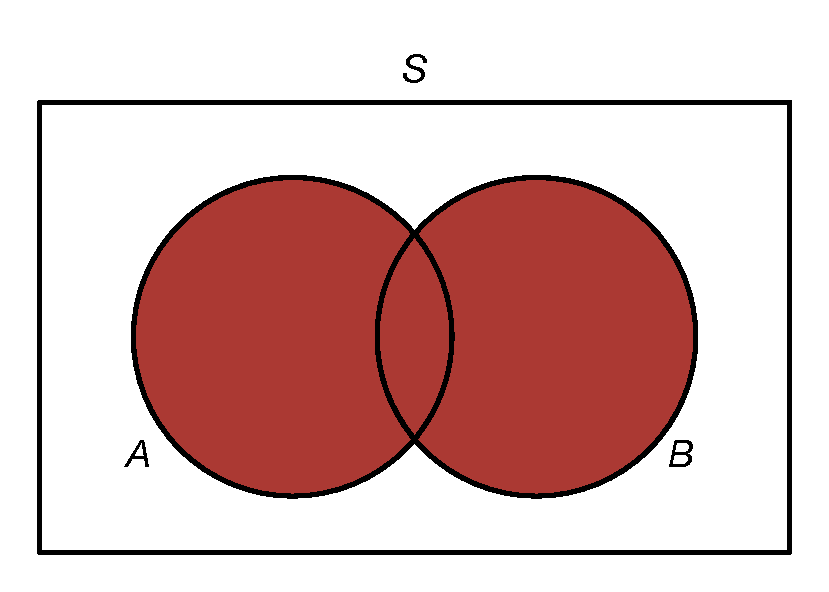
\includegraphics[width=8cm]{AunionB}
\end{figure}
\item The \emph{intersection} of $A$ and $B$, denoted $A \cap B$, is the set of all elements which are in both $A$ and $B$.
\begin{figure}[H]
\centering
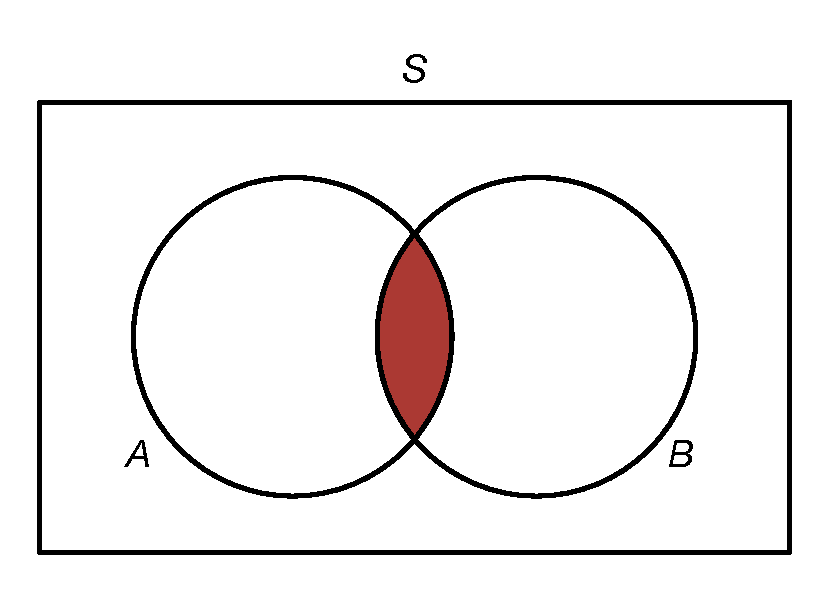
\includegraphics[width=8cm]{AintersectB}
\end{figure}
Two sets $A$ and $B$ are \emph{disjoint} or \emph{mutually exclusive} if they have no elements in common, i.e. if $A \cap B = \emptyset$.
\begin{figure}[H]
\centering
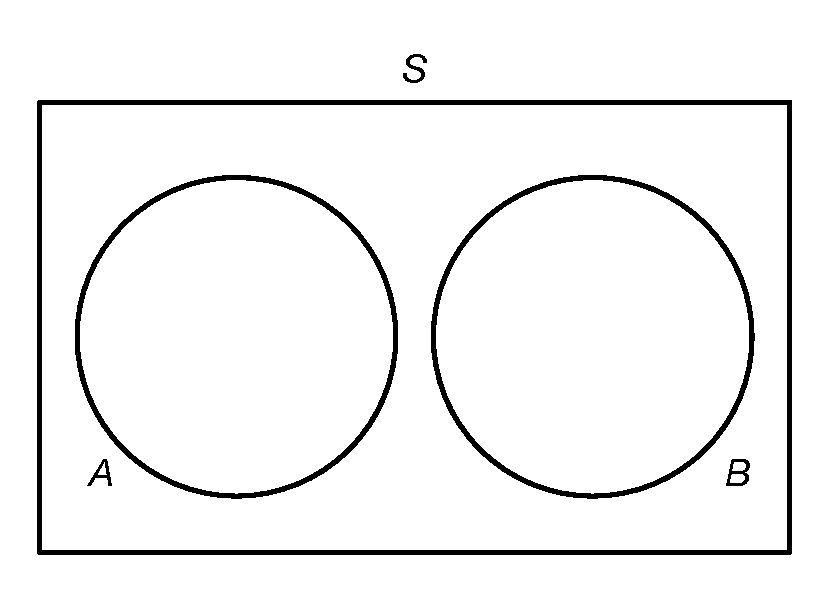
\includegraphics[width=8cm]{exclusive}
\end{figure}
\item The \emph{complement} of $A$, denoted $A^c$, is the set of all points in $\cals$ which are not in $A$. Note that $A$ and $A^c$ are disjoint, and $A \cup A^c = \cals$.
\begin{figure}[H]
\centering
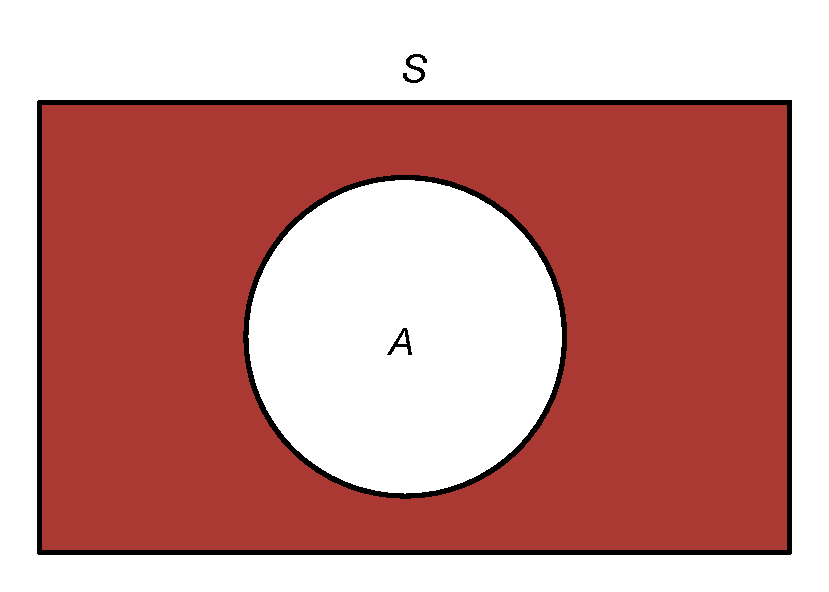
\includegraphics[width=8cm]{Acomplement}
\end{figure}
\end{enumerate}
There are many relationships between these operations which fall under the rubric of set algebra. Most of them we will not need, but we mention a few useful ones here:
\begin{enumerate}
\item Distributive laws
\begin{align*}
A \cap (B \cup C) &= (A \cap B) \cup (A \cap C) \\
A \cup (B \cap C) &= (A \cup B) \cap (A \cup C)
\end{align*}
\item DeMorgan's laws
\begin{align*}
(A \cap B)^c &= A^c \cup B^c &\text{(the complement of an intersection is the union of the complements)}\\
(A \cup B)^c &= A^c \cap B^c &\text{(the complement of a union is the intersection of the complements)}
\end{align*}
\end{enumerate}

\subsection{Axiomatic Definition of Probability}
Equipped with our our knowlege of set theory, we can define probability axiomatically as follows. Given any event $A$ in our sample space $\cals$, we assign a probability $\P(A)$ to that event such that the following rules hold\footnote{You can construct a coherent notion of probabiltiy with fewer axioms and derive the remaining rules from these; I like this version of probability rules, since it codifies what we want to be true given our intuitive notion of probability.}:
\begin{enumerate}
\item $0 \leq \P(A) \leq 1$ \\

The probability of an event is a real number between 0 and 1, where a probability of 0 means that the event will never occur, and a probability of 1 means that the event will always occur.
\item $\P(\emptyset) = 0$ \\

The probability that nothing happens is 0, i.e. something must happen.
\item $\P(\cals) = 1$ \\

The probability of the whole sample space is 1, which is another way of saying that something must happen.
\item If $A \subset B$, then $\P(A) \leq \P(B)$ \\

If we make a set bigger, its probability can only increase (or stay the same); it cannot decrease.

\item If $A_1, A_2, \dots, A_n$ are pairwise disjoint events, i.e. $A_i \cap A_j = \emptyset$ if $i \neq j$, then
\[
\P(A_1 \cup A_2 \cup \cdots \cup A_n) = \sum_{i=1}^n \P(A_i)
\]
This holds for an infinite sequence as well, i.e. if $A_1, A_2, A_3, \dots$ are a sequence of pairwise disjoint events, then 
\[
\P(A_1 \cup A_2 \cup A_3 \cup \cdots) = \sum_{i=1}^\infty \P(A_i)
\]
\end{enumerate}

From these we can derive a very important rule:
\[
\P(A) + \P(A^c) = 1, \:\:\text{ i.e. }\P(A) = 1 - \P(A^c)
\]
Sometimes it is easier to calculate the probability of an event \emph{not} happening than the probability of the event itself!\\

These rules tell us the properties that we want probability to have. However, given a sample space, they do not actually tell us how to assign probabilities to each event in the sample space. Doing that in a way that is consistent with the above rules can be a bit tricky \footnote{In fact, for an uncountable sample space such as $\cals = [0, 1]$, you can show that you cannot construtct a notion of probability which is consistent with all the rules; this is the starting point for the development of measure theory, and is beyond the scope of this course.}, but luckily for a discrete sample space we can do this with no problem. Since a discrete sample space is composed of a finite (or countable) number of simple events, all we have to do is assign probabilities to each simple event in such a way that they all add up to 1.

\begin{example}Consider once again tossing a single die. The sample space for this is $\cals = \{1, 2, 3, 4, 5, 6\}$. This sample space contains 6 simple events: $\{1\}, \{2\}, \{3\},\{4\}, \{5\}$, and $\{6\}$. We can assign any probabilties we want to these simple events, as long as they add up to 1. For example, assuming we have a fair die, we can let $\P(\{i\}) = 1/6$ for $i = 1, \dots, 6$. If we like, we can check that all the above rules hold. If we have a loaded die, which rolls a 6, say, half the time, we could assign probabilites: $\P(\{6\}) = 1/2, \P(\{i\}) = 1/10$ for $i = 1, \dots, 5$.
\end{example}

\begin{example}Consider this time a countable sample space $\cals = \N = \{1, 2, 3, \dots\}$. One possibility is to assign probabilities $\P(\{i\}) = 1/2^i$ for $i = 1, 2, 3, \dots$, i.e. $\P(\{1\}) = 1/2$, $\P(\{2\}) = 1/4$, $\P(\{3\}) = 1/8$, etc. Perhaps you recall from calculus that this is a geometric series with first element $1/2$ and common ratio $1/2$, and so we know its sum is:
\[
\sum_{i = 1}^{\infty} \P(\{i\}) = \sum_{i = 1}^{\infty} \frac{1}{2^i} = \frac{1}{2}\frac{1}{1 - 1/2} = 1
\]
Since the sum of the probabilities of all the simple events is 1, we are all set! If you have not seen this before, we will cover this in more detail when we discuss the geometric distribution. In the meantime, here is a nice picture to convince you that the sum is indeeed 1.
\begin{figure}[H]
\centering
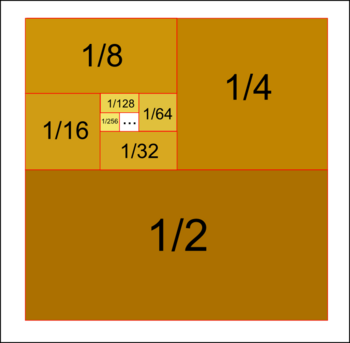
\includegraphics[width=5cm]{Geometric_series}
\end{figure}
\end{example}

% end of class 1
% \end{document}

\subsection{Discrete Uniform Distribution}
The first probability distribution we will consider is the uniform distribution on a \emph{finite} sample space. In the discrete uniform distribution, every simple event is equally likely to occur. \\

Suppose we have a finite sample space $cals$ with $n$ simple events. The discrete uniform distribution assigns each simple event a probability of $1/n$. Why is this the case? If each simple event has probability $p$ and there are $n$ simple events $A_1, \dots A_n$ in our sample space, then using the fact that the sample space $S$ must have probability 1 and that the simple events are pairwise disjoint:
\begin{align*}
1 &= \P(S) \\
&= \P(A_1 \cup A_2 \cup \cdots \cup A_n) \\
&= \P(A_1) + \P(A_2) + \dots + \P(A_n) \\
&= np
\end{align*}
where in the last line we use the fact that the simple events each have probability $p$, and there are $n$ of them. Solving for $p$, we get $p = 1/n$.\\

How do we find the probability of an event that is not a simple event? Again, consider a discrete sample space $\cals$ with $n$ simple events. Suppose we have an event $A$ which is a subset of $\cals$. Since we have a finite sample space, $A$ is composed of a finite number $m$ of simple events, where $m$ is an integer between 0 and $n$. The probability of $A$ is:
\[
\P(A) = \frac{ \text{number of simple events in $A$}}{\text{number of simple events in $\cals$}} = \frac{m}{n}
\]


\begin{example}Consider the finite sample space $\cals$ representing the roll of two standard dice. This sample space has 36 simple events, so each simple event has a probability of 1/36. Note that for the simple events in this sample space, the order of the die rolls matters. $(1, 6)$ and $(6, 1)$ are two different events; even though both events contain the same die rolls, for the former, the 1 is rolled first, while for the latter, the 6 is rolled first.
\begin{enumerate}
\item What is the probability that the sum of the two dice is 7? Looking at the graphical depiction of this event above, we see that there are 6 simple events that give us a sum of 7. Thus the probability of a sum of 7 is 6/36 = 1/6.
\item What is the probability that the sum of the two dice is less than 11. In this case, it is easier to compute the probability that the sum is 11 or greater and then subtract that probability from 1. (Why can we do this?) Let $A$ be the event that the sum is 11 or greater. $A$ is composed of 3 simple events: $(6, 6), (6, 5)$, and $(5, 6)$. Thus we have $\P(A) = 3/36$. The probability we want is:
\[
\P(A^c) = 1 - \P(A) = 1 - 3/36 = 33/36
\]
\end{enumerate}
\end{example}
In the previous example, it is relatively straightforward to draw the sample space, so we can essentially compute any probabily we want simply by looking at the picture and counting which boxes comprise our event of interest. For more complicated problems, this is not as easy. Consider the following example:

\begin{example}A communication system consists of $n$ antennas arranged in a line. Exactly $m$ out of the $n$ antennas are defective. The system is functional if no two consecutive antennas are defective. Assuming that each linear arrangement of the antennas is equally likely, what is the probability that the system will be functional?\\

For small values of $n$ and $m$, say $n = 4$ and $m = 2$, we can write out all of the possible configurations. Representing a functional antenna by \texttt{1} and a defective antenna by \texttt{0}, there are exactly six linear arrangements:
\begin{enumerate}[noitemsep]
\item 0 1 1 0
\item 0 1 0 1
\item 0 0 1 1
\item 1 0 0 1
\item 1 0 1 0
\item 1 1 0 0
\end{enumerate}
Take a moment to convince yourself that these are the only possible configurations. Configurations 1, 2, and 5 are functional, so there are 3 functional configurations out of 6 total configurations. So in this case, the probability that the system is functional is 3/6. \\

For general $n$ and $m$, it is not immediately obvious how to perform the requisite counting of configurations. Taking a cue from the Count on Sesame Street, we need to learn more about counting. The mathematical theory of counting is known as \emph{combinatorics}.
\end{example}

\subsubsection{The Basic Principle of Counting}

\begin{framed}
  \emph{The basic principle of counting ($mn$-rule) }\\
  \rule{\dimexpr\linewidth-2\fboxsep-2\fboxrule}{.1pt} \\
  Suppose we are performing two experiments. If the first experiment has $m$ possible outcomes and the second experiment has $n$ possible outcomes, there are $mn$ possible outcomes for the two experiments. We can generalize this to more than two experiments; in that case, we take the product of the number of outcomes from each experiment.
\end{framed}

To see this, draw a grid of boxes with the $m$ outcomes from the first experiment on the left and the $n$ outcomes of the second experiment across the top. There are $mn$ total boxes, which are all the possible outcomes of both experiments.

\begin{figure}[H]
\centering
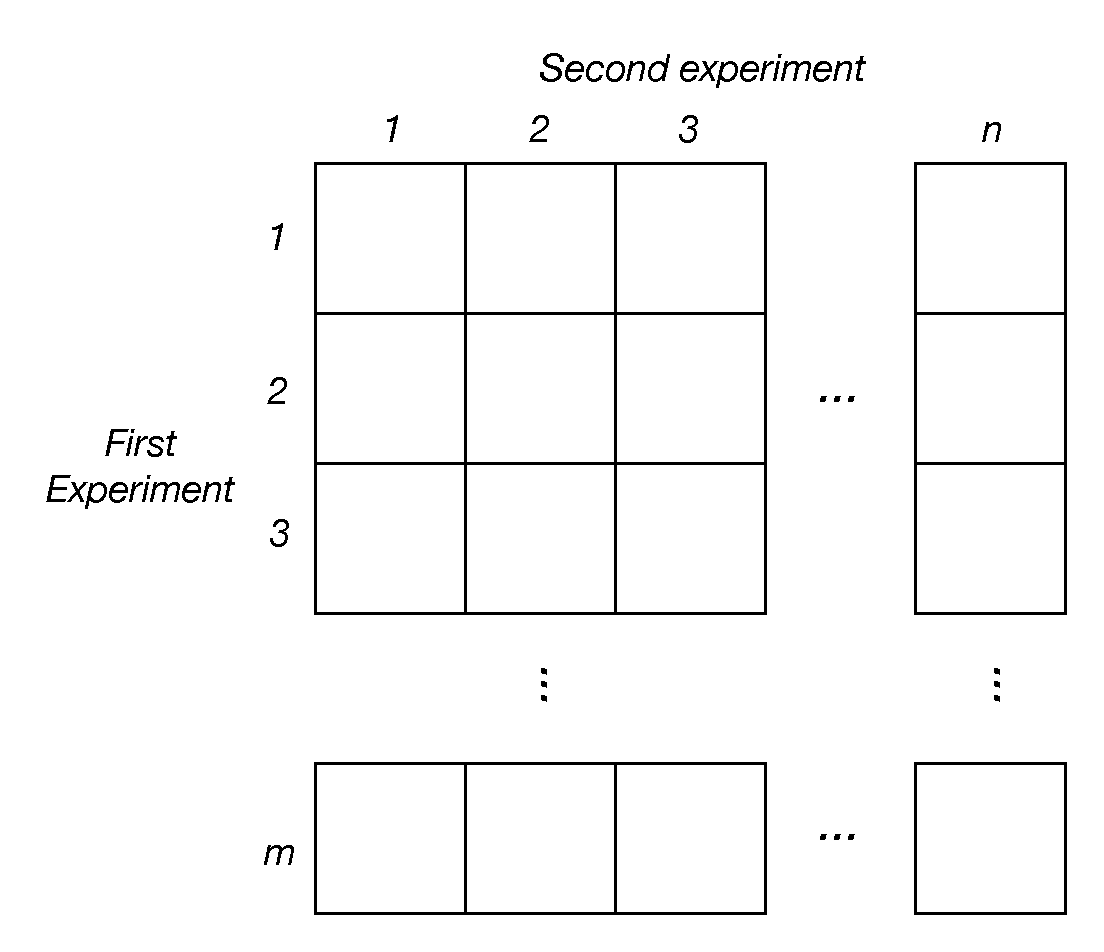
\includegraphics[width=6cm]{mnrule.eps}
\end{figure}

We have already seen the basic principle of counting in play when we looked at the sample space for two dice. Each of the two die rolls is a separate experiement. Since there are 6 outcomes for each die roll, the total number of outcomes is $6 \cdot 6 = 36$. We can extend this to three or more dice. For three dice, for example, the total number of oucomes is $6 \cdot 6 \cdot 6 = 6^3 = 216$. If you like, you can visualize this as a cube. For $n$ dice, there are $6^n$ possible outcomes. I have trouble visualizing this for $n > 3$, but perhaps you can.\\

We can also think of the basic principle of counting in terms of choosing items from groups. If there are $m$ items in Group 1 and $n$ items in Group 2, there are $mn$ pairs of items consisting of one item from each group. Again, this can be extended to any number of groups.\\

\begin{example}When I was growing up in Virginia, standard (non-vanity) license plates were composed of three letters (A-Z) followed by three digits (0-9). Assuming that all such possibilities can exist:
\begin{enumerate}
\item How many possible license plates are there? \\

We are choosing items from 6 groups. The first three groups contain 26 items, and the last three groups contain 10. Thus the number of possibilities is: $26 \cdot 26 \cdot 26 \cdot 10 \cdot 10 \cdot 10 = 17,576,000$. (That works out to a little more than two cars per person.)
\item If the Virginia DMV decided that letters and numbers could not be repeated, how many possible license plates would there be?\\

The difference here is that the group sizes shrink as we choose items. For the letters, the first group has 26 items. The second group only has 25 items, since we cannot choose the letter we chose from the first group. The third group has 24 items, since we cannot choose the letter we chose from the first two groups. The digits are similar. Thus the number of possibilities is: $26 \cdot 25 \cdot 24 \cdot 10 \cdot 9 \cdot 8 = 11,232,000$
\end{enumerate}
\end{example}

\subsubsection{Permutations}

\begin{framed}
An ordered arrangement of $r$ distinct items is called a \emph{permutation}. The number of ways of ordering $r$ items drawn from a group of $n$ distinct items is designated $nPr$.
\end{framed}

Before we give the formula for the number of possible permutations, let's look at some examples so we can get an intuitive understanding of what is going on.

\begin{example}How many different ordered arrangements are there of the letters \emph{a}, \emph{b}, and \emph{c}? \\

In this case, we can actually write them all out: \emph{abc}, \emph{acb}, \emph{bac}, \emph{bca}, \emph{cab}, \emph{cba}.\\
From this we see that there are 6 possible ordered arrangements. We can also do this using the ``choosing-from-groups'' approach. For the first letter, we have 3 to choose from; for the second, we have only 2; and for the third, there is only one remaining letter. Thus the number of permutations is:
\[
3 \cdot 2 \cdot 2 = 3! = 6
\]
Similarly, the number of ordered arrangements of $n$ distinct symbols is:
\[
n \cdot (n-1) \cdot (n-2) \cdots 2 \cdot 1 = n!
\]
The symbol $n!$ is the \emph{factorial} operation, and it is defined exactly as written above.
\end{example}

\begin{example}Every December (since 1996), the city of Ithaca, NY hosts the International Rutabega Curl\footnote{\url{http://www.rutabagacurl.com}} (contestants must supply their own rutabega). Gold, silver, and bronze medals are given to the top three finishers. If 100 contentants enter the rutabega curl, how many possibilities are there for the winners?\\

For the gold medalist, we have 100 contestants to choose from. Since you cannot win more than one medal, we choose from 99 contentants for the silver medal and 98 contestants for the bronze medal. The number of medal possibilities is:
\[
100 \cdot 99 \cdot 98 = 970,200
\]
\end{example}

We can generalize this in the following formula:

\begin{framed}
The number of permutations (ordered arrangements) of $r$ items drawn from a group of $n$ distinct items is:
\[
nPr = n (n-1)(n-2)\cdots(n - r + 1) = \frac{n!}{(n-r)!}
\]
\end{framed}
To see this, there are:
\begin{itemize}
\item $n$ ways to choose the first item
\item $n-1$ ways to choose the second item\\ \\$\cdots$
\item $n - r + 1$ ways to choose the $r$th item
\end{itemize}
Multiply these together to get the permutation formula. To get the ``factorial form'' of the permutation formula, we have:
\[
nPr = n (n-1)(n-2)\cdots(n - r + 1)\frac{(n-r)!}{(n-r)!} = \frac{n!}{(n-r)!}
\]
where $n! = n(n-1)\cdots2\cdot1$, and we define $0! = 1.$\footnote{This may seem a little arbitrary, but it is convenient. It also makes some sense that there is exactly one way to arrange no items.}

\subsubsection{Combinations}
Consider the following example, which is modification of the Rutabega Curl example above.

\begin{example}100 students buy raffle tickets. Three names are chosen from a hat uniformly at random to win a free sandwich at Eastside Pockets\footnote{A popular eatery on Thayer St. near Brown University}. How many possibilities are there for the winners?\\

How is this problem fundamentally different from the Rutabega Curl? Here, the three prizes are identical, as opposed to the three distinct medals in the Rutabega Curl. We can think of this problem as selecting 3 items from a group of 100, but \emph{the order in which we select them does not matter}. Let's look at this in a few stages:
\begin{enumerate}
\item Let's pretend for a moment that the order of selection matters. Then, as in the Rutabega Curl, there are $100 \cdot 99 \cdot 98$ possibilities.
\item Compared to the the case where order matters, is the number of possibilities greater, fewer, or the same? There must be fewer possibilities since, for example, choosing the numbers $(1, 2, 3)$ from the hat in that order is the same as choosing them in the order $(3, 2, 1)$.
\item How many permutations correspond to choosing the numbers 1, 2, and 3 from the hat? We can write out all the permutations:
\[
(1, 2, 3), (1, 3, 2), (2, 1, 3), (2, 3, 1), (3, 1, 2), \text{ and } (3, 2, 1)
\]
This gives us a total of 6 permutations. But this number is $3!$, the number of ordered arrangements of 3 objects. Does this make sense that this should be the case.
\item Since we have shown that 6 permutations correspond to one possibility of winners, all we need to do is divide the number of permutations by 6. Thus the total number of possibilities for the winners is:
\[
\frac{100 \cdot 99 \cdot 98}{6}
\]
\end{enumerate}
\end{example}

\begin{framed}
An unordered arrangement of $r$ distinct items is called a \emph{combination}. The number of combinations of $r$ items drawn from a group of $n$ distinct items is denoted $\binom{n}{r}$ (or sometimes $nCr$). We can think of this as:
\begin{enumerate}
\item The number of subsets of size $r$ which can be formed from a group of $n$ distinct objects
\item The number of ways to select $r$ items from a group of $n$ distinct items, where order does not matter
\end{enumerate}
\end{framed}

Using the logic from the previous example, we can deduce the formula for $\binom{n}{r}$. All we have to do is take the number of permutations and divide by $r!$, which is the number of ordered arrangements (permutations) of $r$ items.

\begin{framed}
The number of combinations (unordered arrangements) of $r$ items drawn from a group of $n$ distinct items is:
\[
\binom{n}{r} = \frac{nPr}{r!} = \frac{n!}{r!(n-r)!}
\]
\end{framed}

\begin{example}The Brown crossword puzzle club consists of 5 undergraduate and 7 graduate students.
\begin{enumerate}
\item How many different committees of 2 undergrads and 3 grad students can be formed?

There are $\binom{5}{2}$ possible groups of 2 undergrads, and $\binom{7}{3}$ possible groups of 3 grad students. We multiply these together (basic principle of counting) to get:
\[
\binom{5}{2} \binom{7}{3}  = \frac{5!}{2!3!} \frac{7!}{3!4!} = \frac{5\cdot4}{2\cdot1} \frac{7\cdot6\cdot5}{3\cdot2\cdot1} = 10 \cdot 35 = 350
\]

\item What if two of the grads students refuse to be on the same committee?

There are $\binom{7}{3} = 35$ possible groups of 3 graduate students. How many contain both of the two students who refuse to serve together? To make a three-person committee which includes these two, you need to include the two rival students plus one other student selected from the five remaining graduate students. Thus there are $\binom{2}{2}\binom{5}{1} = 5$ committees which include the two rival students. Subtracting from 35, there are 30 committees which don't include both rival students. As above, we multiply to get $10 \cdot 30 = 300$ possible committees.
\end{enumerate}
\end{example}

Computing probabilities of poker hands are classic problems in probability. Since the order of the cards in a poker hand does not matter, these problems involve combinations.

\begin{example}
You are dealt a five-card poker hand. What is the probability of getting a full house (three cards of one number plus two cards of another number)\\

There are 52 cards in a poker deck, and a poker hand is 5 cards. Since the order of the cards dealt does not matter, there are $\binom{52}{5}$ possible five-card poker hands. To count the number of hands which give us a full house, we use the following procedure:
\begin{enumerate}
\item Choose the number for the three-of-a-kind. There are $\binom{13}{1}$ ways to do that. Now select three out of the four cards of this number. There are $\binom{4}{3}$ ways to do that. Thus there are $\binom{13}{1}\binom{4}{3}$ ways to choose the three-of-a-kind.
\item Choose the number for the pair. There are $\binom{12}{1}$ ways to do that, since we have already chosen one of the numbers for the three-of-a-kind. Now select two out of the four cards of this number. There are $\binom{4}{2}$ ways to do that. Thus there are $\binom{12}{1}\binom{4}{2}$ ways to choose the pair once the three-of-a-kind has been chosen.
\item Multiply all of these together to get $\binom{13}{1}\binom{4}{3}\binom{12}{1}\binom{4}{2}$ poker hands which are full houses.
\end{enumerate}
To get the probability of a full house, we divide by the number of poker hands (the size of the sample space) to get:
\[
\frac{\binom{13}{1}\binom{4}{3}\binom{12}{1}\binom{4}{2}}{\binom{52}{2}} = 0.00144
\]
It is worth noting that the number of full houses is not $\binom{13}{2}\binom{4}{3}\binom{4}{2}$, i.e. choose two numbers, then choose a three-of-a-kind, then choose a pair. Why does this not work? This method does not distinguish betwen, say, \texttt{33366} and \texttt{33666} (i.e. it treats these as the same), and these are two distinct full houses. Since this undercounts by a factor of two, you can check that if you multiply this by two, you get the correct answer above. 
\end{example}

Combinations are incredibly useful. We can use them in some rather surprising cases.

\begin{example}Consider the binary string \texttt{11000}. How many distinct orderings are there of the digits in this string?\\

At first, this does not appear to involve combinations at all, since we are looking for orderings, and combinations are used where order does not matter. Let's look at this problem in a different way. Consider the five-element set $A = \{a, b, c, d, e\}$. There are $\binom{5}{2}$ two-element subsets of $A$. One way to describe subsets of $A$ is to make a table. The columns of the table represent the elements of $A$: $a, b, c, d$, and $e$. Each row corresponds to a subset of $A$: a 1 indicates that the element is in the subset, and a 0 indicates that it is not. Here is an example table, where we depict two two-element subsets.

\begin{figure}[H]
\centering
\label{twoelementsubsets}
\begin{tabular}{lllll|l}
$a$ & $b$ & $c$ & $d$ & $e$ & subset \\
\hline
0 & 0 & 1 & 1 & 0 & $\{c, d\}$\\
1 & 0 & 1 & 0 & 0 & $\{a, c\}$\\
\end{tabular}
\end{figure}

Notice that two-element subsets match up exactly with orderings of \texttt{11000}! Thus we see that there are $\binom{5}{2}$ rearrangements of the binary string \texttt{11000}.
\end{example}

In general, if you have a string of length $n$ composed of two symbols, and you have $r$ of one symbol (thus $n-r$ of the other), the number of distinct orderings of the string is $\binom{n}{r}$. Equipped with this, let's return to the antenna example from the beginning of the section.

\begin{example}A communication system consists of $n$ antennas arranged in a line. Exactly $m$ out of the $n$ antennas are defective. The system is functional if no two consecutive antennas are defective. Assuming that each linear arrangement of the antennas is equally likely, what is the probability that the system will be functional?\\

First we need to figure out how many possible arrangements there are, i.e. the size of our sample space. If we use the digit \texttt{1} to represent a functional antenna, and the digit \texttt{0} to represent a defective antenna, then each arrangement can be represented by a binary string of length $n$ consisting of $m$ 0s and $n - m$ 1s. Thus from what we learned above, there are $\binom{n}{m}$ possible arrangements. \\

How many of these arrangements are functional? Let's draw a picture! Imagine we have the $n - m$ functional antennas in a line. We will represent each functional antenna by the symbol *, and the spaces between the functional antennas by a vertical bar $|$. We will also place a space to the far right and to the far right:
\[
| * | * | * | * | * | * | \dots | * | * |
\]
For the system to be functional, each space $|$ can contain at most one defective antenna. There are $n - m + 1$ spaces to choose from, and $m$ defective antennas to place. Thus there are $\binom{n-m+1}{m}$ functional arrangements. Dividing this by the total number of arrangements $\binom{n}{m}$, the probability that the system is functional is:
\[
\frac{ \binom{n-m+1}{m}}{\binom{n}{m}}
\]
For a sanity check, let's calculate this for the case where $n = 4$ and $m = 2$, which we did manually above:
\[
\frac{ \binom{n-m+1}{m}}{\binom{n}{m}} = \frac{\binom{3}{2}}{\binom{4}{2}} = \frac{3}{6} = \frac{1}{2}
\]
\end{example}
This agrees with what we found above!

\begin{example}
I buy an assortment of 10 bagels from Bagel Gourmet on Thayer St.\footnote{Having lived in Brooklyn for many years, I am only \emph{slightly} obsessed with bagels.}. There are five types of bagels to choose from: everything, onion, poppy, raisin, and sesame. How many different assortments of bagels can I bring home? Assume there are at least 10 of each kind of bagel in the store.\\

We can model the problem in a way that lets us use combinations. Imagine you buy the bagels in a special box. The bagels are arranged in a line, and are always in alphabetical order: everything, onion, poppy, raisin, sesame. There are four dividers, one between each bagel type, and if a bagel type is not present, we just put the dividers next to each other. Here is an example of three bagel boxes with their dividers. Bagels are designated by * and dividers by $|$.
\begin{figure}[H]
\begin{tabular}{ll}
$* * | * | * * * | * * | * *$ & 2 everything, 1 onion, 3 poppy, 2 raisin, 2 sesame \\
$* * * | | * * * | | * *$ & 3 everything, 3 poppy, 2 sesame\\
$* * * * * * * * * * | | | |$ & 10 everything\\
\end{tabular}
\end{figure}
From the picture, we see that an assortement of 10 bagels can be represented as a linear string of 14 symbols: 10 * representing the bagels and 4 $|$ representing the dividers. The number of assortments is the same as the number of distinct orderings of this linear string: $\binom{14}{4} = 1001$
\end{example}

% end of class 2

One final application of combinations is to the binomial theorem. The binomial theorem gives us a nice expression for expanding the binomial $(x+y)^n$, where $n$ is a positive integer.

\begin{framed}
\emph{The binomial theorem}\\
  \rule{\dimexpr\linewidth-2\fboxsep-2\fboxrule}{.1pt} \\
\[
(x+y)^n = \sum_{r=0}^n \binom{n}{r}x^r y^{n-r}
\]
\end{framed}
Due to their appearance in this theorem, the coefficients $\binom{n}{r}$ are often called \emph{binomial coefficients}. Rather than give the usual proof by induction, we will argue this is true using what we know about combinations. Consider the product:
\[
(x_1 + y_1)(x_2 + y_2)\cdots(x_n + y_n)
\]
If we multiply this out, we get a sum of $2^n$ terms, each of which is the product of $n$ factors. To see this is the case, to get a term in the sum, we pick either $x_i$ or $y_i$ from each of the $n$ binomials $(x_i + y_i)$ and multiply them together. There are $2^n$ such terms, since for each binomial we have two possible choices and there are $n$ total binomials. How many of these $2^n$ terms have exactly $r$ of the $x_i$ terms and $n-r$ of the $y_i$ terms? We can think of each term as a string of length $n$ composed of $r$ $x$'s and $n-r$ $y$'s. By what we learned above, there are $\binom{n}{r}$ such terms. Taking $x_i = x$ and $y_i = y$ for all $i$, we obtain the binomial theorem.

\subsubsection{Multinomials}
\begin{framed}
The number of ways of dividing $n$ objects into $k$ distinct groups containing $n_1, \dots, n_k$ objects each, where each object appears in exactly one group, and $n_1 + \cdots + n_k = n$ is given by:
\[
\binom{n}{n_1 \: n_2\: \cdots \:n_k} = \frac{n!}{n_1!\:n_2!\:\cdots\:n_k!}
\]
The term on the left is called a \emph{multinomial coefficient}
\end{framed}
Note that this is the same as the binomial coefficient when $k = 2$. To see why this is true, we will use the following argument:
\begin{enumerate}
\item For the first group, we choose $n_1$ out of $n$ items. Since order does not matter, there are $\binom{n}{n_1}$ ways to do this.
\item For each choice in step 1, there are $\binom{n - n_1}{n_2}$ choices for the second group, since we have already taken $n_1$ items out of the larger group.
\item For each choice in step 1 and step 2, there are $\binom{n - n_1 - n_2}{n_3}$ choices for the third group, since we already have taken $n_1 + n_2$ items out of the larger group.
\item Repeat this until we get to the $k$th group, where there are $\binom{n - n_1 - \dots - n_{k-1}}{n_k}$ choices for the $k$th group given all the previous choices
\item Multiply these together to get:
\begin{align*}
&\binom{n}{n_1 \: n_2\: \cdots \:n_k} = \binom{n}{n_1} \binom{n - n_1}{n_2} \binom{n - n_1 - n_2}{n_3} \cdots \binom{n - n_1 - \dots - n_{k-1}}{n_k} \\
&= \frac{n!}{n_1! (n - n_1)!}\:\frac{(n - n_1)!}{n_2!(n - n_1 - n_2!)}\:\frac{(n - n_1 - n_2)!}{n_3!(n - n_1 - n_2 - n_3!)}\cdots\frac{n - n_1 - \dots - n_{k-1}!}{n_k! (n - n_1 - \dots - n_k)!}\\
&= \frac{n!}{n_1! \: n_2! \: n_3! \cdots n_k! (n - n_1 - \dots - n_k! )} \\
&= \frac{n!}{n_1! \: n_2! \: n_3! \cdots n_k! \: 0! } \\
&= \frac{n!}{n_1! \: n_2! \: n_3! \cdots n_k! }
\end{align*}
\end{enumerate}
where, after some very satisfying cancellation, we have used the fact that $n_1 + \dots + n_k = n$ and $0! = 1$.\\

If you want to think about this another way, you can use the following reasoning. Imagine we have $n$ objects and want to divide them into groups as above. Imagine we have a special box which contains the $n$ objects in a line. Divide the box into sections using dividers, so that the first section contains $n_1$ objects, the second $n_2$ objects, all the way down to the $k$th section which contains $k$ objects. For example, if we had $n = 10$ with four groups $n_1 = 2, n_2 = 4, n_3 = 1, n_4 = 3$, our box looks like:
\[
* * | * * * * | * | * * *
\]
where * represents a space to put an objects, and $|$ is a section divider. There are $n!$ permutations of $n$ objects, thus there are $n!$ distinct ways to place the $n$ objects into the box. Since we are dividing our objects into groups, order does not matter within each group. The first section in the box represents the first group, so since order does not matter within that section, we divide by $n_1!$, the number of permutations of $n_1$ objects. Repeating this for each section, we divide by each $n_i!$ in turn to obtain our multinomial coefficient. 

\begin{example}A group of 15 international relations students will be divided into three groups. Each group consists of 15 students and is assigned a different country (Azerbaijan, Belarus, and Chechnya) on which to do a group final presentation. How many such divisions are possible:\\

Since we are are dividing 15 people into 3 distinct groups of 5, we can use the multinomial coefficient to determine the number or arrangements:
\[
\binom{15}{5 \: 5\: 5} = \frac{15!}{5!\:5!\:5!} = 756,756
\]
\end{example}

\begin{example}Now suppose we are dividing a group of 15 international relations students into three groups of 5 students each for a final project of the each group's choosing. How is this problem different from the previous one? How many different arrangements are possible?\\

In the previous example, the three groups were distinct, so it matters which one a student is assigned to. In this case, the three groups are identical. Thus since the order of the three groups does not mater, we divide the previous result by $3!$, which is the number of ways of ordering three items (in this case, the items are the three groups).
\[
\frac{ \binom{15}{5 \: 5\: 5}}{3!} = \frac{15!}{5!\:5!\:5!\:3!} = 126,126
\]
\end{example}

\begin{example}How many different, distinct rearrangements are there of the word MISSISSIPPI?\\

We are looking for all distinct orderings of a string with four distinct symbols. If there were only two distinct symbols, we could use binomial coefficients, so we suspect multinomial coefficients may be in play here. Once again, consider a set with eleven elements in them, which we will label with the integers 1 - 11. We want to divide those elements into four subsets with 1, 2, 4, and 4 elements (respectively). We will label those subsets by the letters M, P, I, and S (no coincidence here!). Let's make a table, where each row is a subset, and letters M, I, S, and P in the row indicate which subset each element belongs to.

\begin{figure}[H]
\centering
\label{mississippi}
\begin{tabular}{lllllllllll}
$1$ & $2$ & $3$ & $4$ & $5$ & $6$ & $7$ & $8$ & $9$ & $10$ & $11$ \\
\hline
M & I & S & S & I & S & S & I & P & P & I \\
I & S & I & P & M & P & S & I & S & S & I \\
\end{tabular}
\end{figure} 

Note that there is a perfect correspondance between each appropriate collection of four subsets and each arrangement of MISSISSIPPI. Thus we can use the multinomial coefficient for this problem, and we get that the total number of distinct rearrangements is:
\[
\binom{11}{1 \: 2\: 4 \: 4} = \frac{11!}{1!\:2!\:4!\:4!} = 34,650
\]
\end{example}

\subsection{Conditional Probability}
Sometimes the probability of an event will depend on whether or not another event has occurred. There are many real-life examples of this:
\begin{enumerate}
\item In weather prediction, the probability of rain tomorrow depends on whether or not it is raining today. This especially makes sense during the tropical storm season when it will often rain for days on end.
\item In the field of public health, probabilties of developing disease depend on many outside factors. The probability of developing lung cancer, for example, depends on factors such as smoking history, exposure to second-hand smoke, and occupational exposure to asbestos.
\item Poker players are constantly thinking about conditional probability. For example, what is the probability of an inside straight draw on the final two cards given the cards the player has already seen?
\end{enumerate}

Let's do a simple die-tossing example, and then generalize.

\begin{example}On a standard, fair six-sided die, the probability of rolling a 1 is 1/6. This is the \emph{unconditional probability} of rolling a 1, since this probability does not depend on any additional information. Now suppose we know that our die roll is odd. What is the \emph{conditional probability} of rolling a 1 given the die roll is odd? There are 3 possible odd rolls: 1, 3, and 5. We reduce our sample space to the three odd rolls since we know one of those occurred. Since we still have a discrete uniform distribution, each of the three odd rolls is equally likely. Thus the probability of rolling a 1 given an odd roll is 1/3.
\end{example}

Note that what we did above is reduce our sample space from all six possible rolls to the three odd rolls. We then kept the uniform distribution on the the new, smaller sample space. To generalize this to arbitrary events, let's draw a picture! Let $\cals$ be our sample space, and consider two events $A$ and $B$ in $\cals$. 

\begin{figure}[H]
\centering
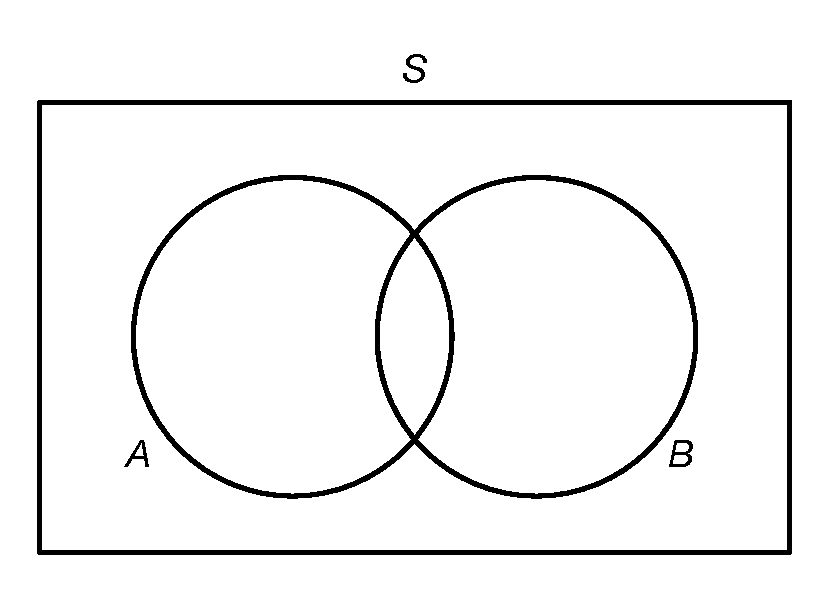
\includegraphics[width=6cm]{venn.eps}
\end{figure}

We are interested in the probability of $A$ given that $B$ has occurred, which we will write $\P(A|B)$ (``the probability of $A$ given $B$''). If $\P(B) = 0$, i.e. $B$ cannot occur, then $\P(A|B)$ must also be 0 (does this make sense?) So we are only interested in the case where $\P(B) > 0$, i.e. $B$ can actually happen. What we are going to do is \emph{restrict} our sample space from $\cals$ down to $B$ since the only events we care about are ones where $B$ has occurred. Imagine taking an eraser (or digital equivalent) to the picture above and removing everything that is outside of B. We are left with the following picture:

\begin{figure}[H]
\centering
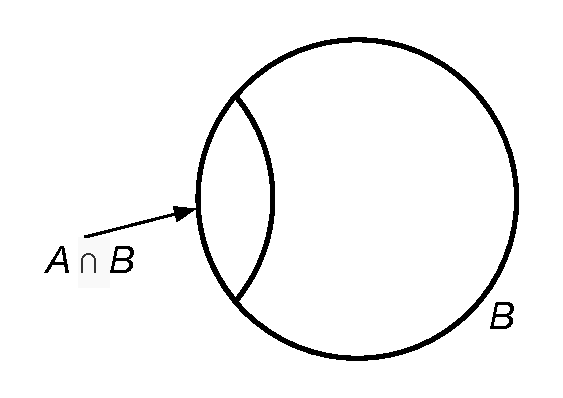
\includegraphics[width=6cm]{AgivenB.eps}
\end{figure}

The piece of $A$ which lies inside $B$ is $A \cap B$, which is on the left of the picture above. If we think of probability intuitively as ``area'' in pictures like this, it makes sense that the conditional probability of $A$ given $B$ is the ratio of $\P(A \cap B)$ to $\P(B)$.

\begin{framed}
Let $A$ and $B$ be two events. The \emph{conditional probability} of $A$ given that $B$ has occurred is given by:
\[
\P(A|B) = \frac{\P(A \cap B)}{\P(B)}
\]
as long as $\P(B) = 0$. (If $\P(B) = 0$, then this is zero.)
\end{framed}

As a sanity check, let's use this definition of conditional probability and redo our die roll example from above.

\begin{example}What is the probability of rolling a 1 on a standard six-sided die given than an odd number was observed?\\

Let $A$ be the event that a 1 is rolled, and $B$ the event that an odd number is rolled. Since $A \subset B$, $A \cap B = A$ (does this make sense?) Using the discrete uniform distribution, $\P(A) = 1/6$ and $\P(B) = 1/2$ (since $B$ is composed of three simple events, each with probability 1/6).
Thus we have:
\[
\P(A|B) = \frac{ \P(A \cap B)}{\P(B)} = \frac{\P(A)}{\P(B)} = \frac{(1/6)}{(1/2)} = \frac{1}{3} \approx 0.339
\]
This agrees with our intuitive computation above.
\end{example}

Let's do another example, this time using the roll of two dice.

\begin{example}
You roll two standard, fair six-sided dice. What is the the probability that the sum is greater than or equal to 11, given that the first roll is a 6?\\

Let $A$ be the event that the sum is greater than or equal to 11, and $B$ the event that the first roll is a 6. The events are shown graphically below.
\begin{figure}[H]
\centering
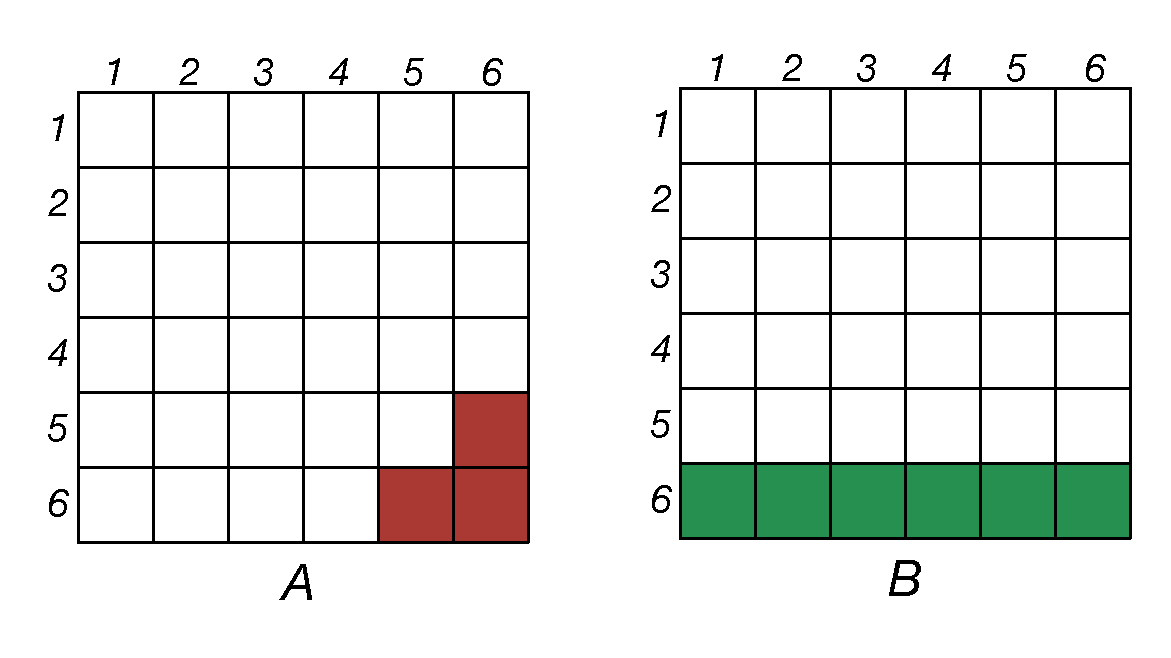
\includegraphics[width=8cm]{2dice1.eps}
\end{figure}
First let's use the sample space reduction method. Given that $B$ has occurred, i.e. the first roll is a 6, we reduce our sample space to $B$, i.e. to the bottom row of the picture. There are six squares in the bottom row, and since we still have the uniform distribution, each is equally likely. Of those 6, 2 of them (the rightmost two) have a sum of dice greater than or equal to 11. Thus the conditional probabaility is $\P(A|B) = 2/6 = 1/3$.\\

We can also use our definition of conditional probabiltiy. Using the uniform distribution, $\P(B) = 6/36$. Since $A \cap B$ is the two rightmost square on the bottom row, $\P(A \cap B) = 2/36$. By the definition of conditional probability:
\[
\P(A|B) = \frac{ \P(A \cap B)}{\P(B)} = \frac{2/36}{6/36} = \frac{1}{3}
\]
Thus again we get the same answer using either method.
\end{example}

Sometimes using a reduced sample space is much easier that using the definition of conditional probabiltiy. Consider the following example.

\begin{example}In the card game bridge (which is near and dear to my heart), 52 cards are dealt out equally to 4 players (called North, South, East and West). Given that North and South have a total of 8 spades between them (out of 13 total spades), what is the probability that East has 3 spades.\\

Here it is easiest to work with a reduced sample space. If North and South have 26 cards and 8 spades between them, then East and West much have the remaining 26 cards and 5 spades between them. The reduced sample space we will work with is the sample space of possible hands for East. Since East has 13 of the remaining 26 cards, there are $\binom{26}{13}$ possible hands for East. This is the size of the sample space. In how many of those hands does East have exactly 3 spades? To do this, we first choose 3 of the remaining 5 spades. There are $\binom{5}{3}$ ways to do this. Then we need to choose the non-spade cards. East has 10 non-spade cards, and there are $26 - 5 = 21$ non-spade cards to choose from, thus there are $\binom{21}{10}$ ways to choose these. Multiplying these together, there are $\binom{5}{3}\binom{21}{10}$ possible hands where East has exactly 3 of the remaining spades. Thus the conditional probability that East has 3 spades given that North and South have 8 spades between them is:
\[
\frac{ \binom{5}{3}\binom{21}{10} }{\binom{26}{13}} \approx 0.339
\]
\end{example}

\subsection{Independence}
Two events $A$ and $B$ are independent if the whether or not one event occurs is unaffected by whether or not the other event occurs. We will make this mathematically precise in a momement, but here are some intuitive examples:
\begin{enumerate}
\item You are flipping coins repeatedly. Each coin flip is independent of all other coin flips, since there is no way for coin flips to affect each other. Now imagine you flip 10 heads in a row. It is tempting to say that the streak of heads must break, and that it is more likely than not that the 11th flip is a tail. This is known as the \emph{gambler's fallacy}, and is false since the flips are independent, and each flip has a 1/2 probability of heads. A famous example of this occurred in the Monte Carlo casino in Monaco on August 18, 1913. In a game of roulette, the ball landed on black 26 times in a row, and gamblers lost a lot of money betting that the streak would break.
\item In blackjack, if a player is dealt an ace, the next deal is less likely to be an ace, since the cards are drawn without replacement. Successive deals of cards are thus not independent. This is the basis for counting cards in blackjack and other games.
\item In the field of public health, ``smoking'' and ``contracting lung cancer'' are not independent since a causal link has been shown between the two.
\end{enumerate}
We are ready to formally definite the concept of independence.

\begin{framed}
Let $A$ and $B$ be two events. $A$ and $B$ are \emph{independent} if any of the following hold:
\begin{align*}
\P(A|B) &= \P(A) \\
\P(B|A) &= \P(B) \\
\P(A \cap B) &= \P(A)\P(B)
\end{align*}
In plain language, two events are independent if the conditional probability is the same as the unconditional probability, or if the probability of both events occurring is the same as the product of the probabilities of the individual events.
\end{framed}

Let's look at a few examples of independence.

\begin{example}
Let us roll a single fair, six-sided die, and consider the following events:
\begin{itemize}
\item $A$: we roll an odd number
\item $B$: we roll an even number
\item $C$: we roll a 1 or a 2
\end{itemize}
\begin{enumerate}
\item Are $A$ and $B$ independent? \\

Because $A \cap B = \emptyset$, $\P(A \cap B) = 0$, thus $\P(A|B) = \P(A \cap B) / \P(B) = 0$. But $\P(A) = 1/2$. Since $\P(A|B) \neq \P(A)$, $A$ and $B$ are not independent. We did not expect them to be independent, since if $A$ occurs, $B$ cannot occur, and vice versa.
\item Are $A$ and $C$ independent? \\

Using the sample space reduction method, we see that $\P(A|C) = 1/2$, since if we know we roll a 1 or a 2, half the time we will roll an odd number. Since $\P(A) = 1/2$ as well, $\P(A|C) = \P(A)$, thus $A$ and $C$ are independent.
\end{enumerate}
\end{example}

For our next problem we revisit our familiar two-coin-flip example.

\begin{example}
Let us roll two fair, six-sided dice, and consider the following events:
\begin{itemize}
\item $A$: we roll a 4 on the first die
\item $B$: the sum of the two dice is 6
\item $C$: the sum of the two dice is 7
\end{itemize}
\begin{enumerate}
\item Are $A$ and $B$ independent? \\

Here we use the ``product of probabilites'' test for independence. $\P(A \cap B) = 1/36$, since if we know the first die is 4 and the two dice sum to 6, the second die must be a 2; this corresponds to a single point in the sample space. $\P(A) = 1/6$, since a single die has a 1/6 chance of rolling any number. $B$ comprises 5 simple events, as we can see graphically below; thus $\P(B) = 5/36$. 
\begin{figure}[H]
\centering
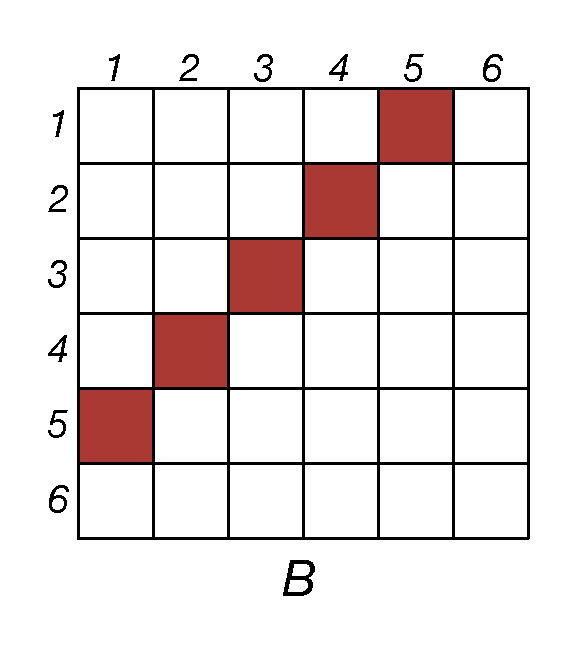
\includegraphics[width=4cm]{2dice2.eps}
\end{figure}
Since $\P(A)\P(B) = (1/6)(5/36) = 5/216 \neq 1/36 = \P(A \cap B)$, these events are not independent. Why does this make sense? If we are interested in a sum of 6 on two dice, the outcome of the first throw matters; a sum of 6 is impossible if the first die is a 6, and is possible for all other rolls of the first die. Thus is makes sense that $A$ and $B$ should not be independent.

\item Are $A$ and $C$ independent? \\

Here, we have again that $\P(A \cap C) = 1/36$, since if we know the first die is 4 and the two dice sum to 7, the second die must be a 3; $\P(A) = 1/6$ as above. We can see graphically that $\P(C) = 6/36 = 1/6$, since $C$ comprises 6 simple events. Thus $\P(A)\P(C) = (1/6)(1/6) = 1/36 = \P(A \cap C)$, and so $A$ and $C$ are independent. Why does this make sense? No matter what we roll on the first die, there is an equal probability (1/6) of getting a sum of 7 when the second die is rolled.
\end{enumerate}
\end{example}

\subsection{Multiplicative and Additive Laws of Probability}
The multiplicative and additive laws of probability give the probabilties of intersections and unions of events, and are important in constructing probabilies for more complicated events.

\begin{framed}
\emph{The multiplicative law of probability}\\
  \rule{\dimexpr\linewidth-2\fboxsep-2\fboxrule}{.1pt} \\
Let $A$ and $B$ be two events. Then the probability of the intersection of the two events is:
\begin{align*}
\P(A \cap B) &= \P(A)\P(B|A) \\
&= \P(B)\P(A|B)
\end{align*}
If $A$ and $B$ are independent, then:
\[
\P(A \cap B) = \P(A)\P(B)
\]
\end{framed}
This follows directly from the definition of conditional probability. We can extend this to find the probability of the intersection of multiple events. For example, for three events $A$, $B$, and $C$, we have:
\[
\P(A \cap B \cap C) = \P(A)\P(B|A)\P(C|A\cap B)
\]
We can extend this string of conditional probabilities to find the probability of the intersection of as many events as we want. \\



The additive law of probability gives the probability of the union of two events.
\begin{framed}
\emph{The additive law of probability}\\
  \rule{\dimexpr\linewidth-2\fboxsep-2\fboxrule}{.1pt} \\
Let $A$ and $B$ be two events. Then the probability of the union of the two events is:
\begin{align*}
\P(A \cup B) &= \P(A) + \P(B) - \P(A \cap B) 
\end{align*}
If $A$ and $B$ are disjoint (mutually exclusive), i.e. $\P(A \cap B) = \emptyset$, then:
\[
\P(A \cup B) = \P(A) + \P(B)
\]
\end{framed}

To see this is true, consider the Venn diagram below.
\begin{figure}[H]
\centering
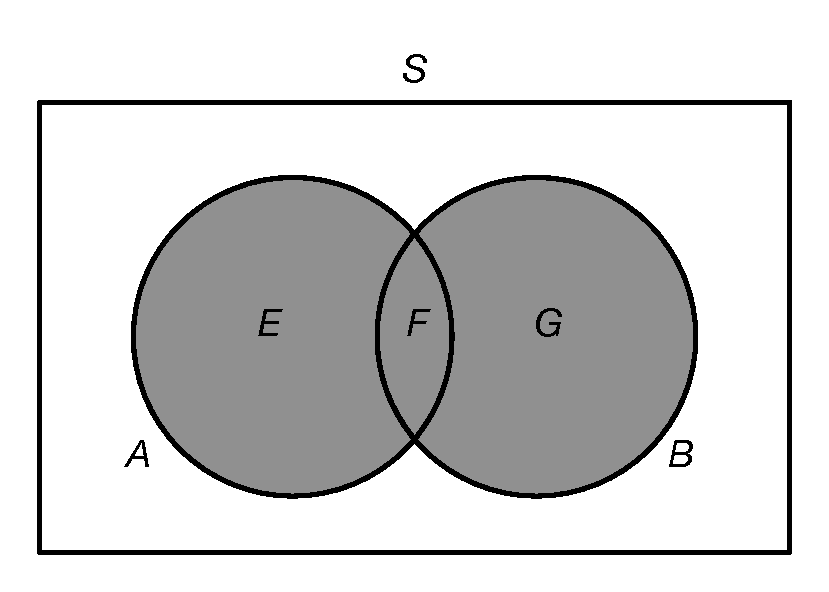
\includegraphics[width=6cm]{additive.eps}
\end{figure}
\begin{enumerate}
\item $A \cup B$ (show in gray) is the disjoint union of $E$, $F$, and $G$, so by the additive property of probability, $\P(A \cup B) = \P(E) + \P(F) + \P(G)$.
\item $A$ is the disjoint union of $E$ and $F$, so by $\P(A) = \P(E) + \P(F)$.
\item $B$ is the disjoint union of $F$ and $G$, so by $\P(B) = \P(F) + \P(G)$.
\item Addding together $\P(A)$ and $\P(B)$, and noting that $F = A \cap B$:
\begin{align*}
\P(A) + \P(B) &= \P(E) + \P(F) + \P(F) + \P(G) \\
&= \P(A \cup B) + \P(A \cap B)
\end{align*}
Rearranging this, we get the additive rule.
\end{enumerate}
Intuitively, if we add the probability of $A$ and $B$, we are ``double-counting'' $A \cap B$, so we have to subtract it off to get $\P(A \cup B)$. This can be extended to unions of more than two sets, but the formulas are annoying and will not be useful to us in this course. 

We can use the multiplication and addition rules in the following problem.

\begin{example}You have two bags of balls. The first bag contains one red ball and three white balls. The second bag contains two red balls and two white balls. You choose a bag uniformly at random and then draw a ball from the chosen bag.
\begin{enumerate}
\item What is the probability that the ball you draw is red?\\

We can do this directly using the multiplication and addition rules if we wish, but it is far easier to draw a \emph{tree diagram}. Let $B_1$ be the event that we choose Bag 1, and $B_2$ the event that we choose Bag 2. Let $R$ be the event that we draw a red ball, and $W$ be the event that we draw a white ball. Then we have the following tree diagram. 
\begin{figure}[H]
\centering
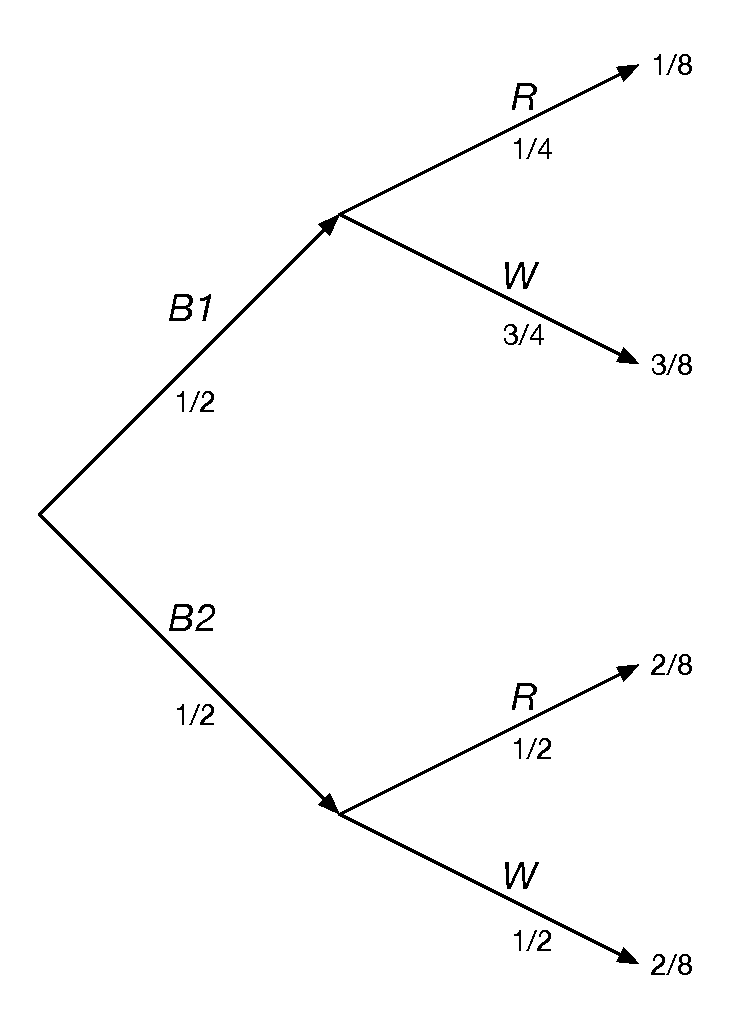
\includegraphics[width=7cm]{tree1.eps}
\end{figure}

Tree diagrams are really hard to explain in writing, but I will try. Starting at the node on the left, the first two edges of the tree are $B_1$ and $B_2$. Their respective probabilities are written below, and are both 1/2, since the choice of bag is uniform. At the point, the tree branches again. Let's look at the top of the tree diagram, the part which follows $B_1$. The upper branch is labeled $R$, and indicates that the event $R$ follows $B_1$. The probability listed there is the conditional probability of $R$ given $B_1$, so $\P(R|B_1) = 1/4$. If we follow the arrows through $B_1$ and $R$, we reach the leaf of the tree which is labeled 1/8. This leaf represents the event $B_1 \cap R$, since we passed through both of those events to get there. The probability 1/8 listed there is the probability of $B_1 \cap R$. We get this by multiplying all the probabilties we passed through to get there. This follows the multiplication rule, since:
\[
\P(B_1 \cap R) = \P(B_1)\P(R|B_1) = (1/2)(1/4) = 1/8
\]
The interpretation of the other branches of the tree is similar. Here is a version of the tree diagram with all the probabilites (conditional and otherwise) labeled: 
\begin{figure}[H]
\centering
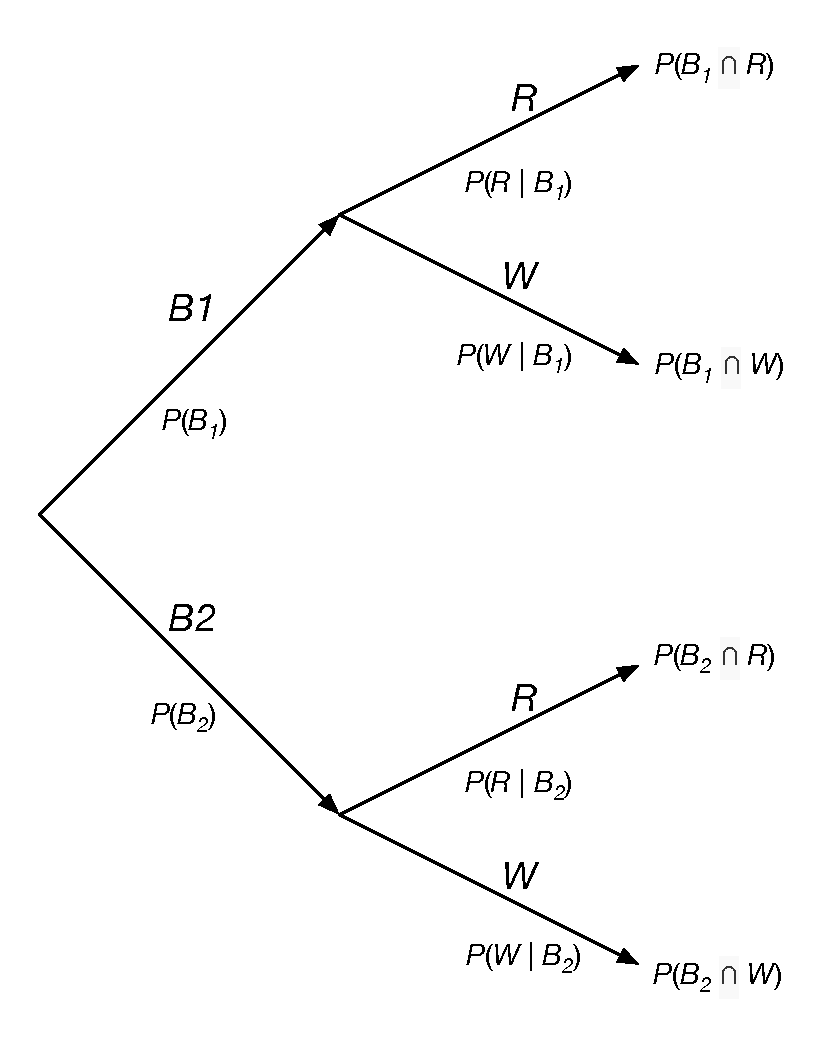
\includegraphics[width=7cm]{tree2.eps}
\end{figure}

To find $\P(R)$, we just add up all the leaves that end passing through $R$. There are two such leaves, labeled with probabilities 1/8 and 2/8, thus $\P(R) = 1/8 + 2/8 = 3/8$.\\

In adding the probabilties above, we used the addition rule. To see how we used it, recall that the sample space is designated $\cals$ and that $B_1$ and $B_2$ are disjoint with $B_1 \cup B2 = \cals$ (you can only choose one bag, and you must choose a bag):
\begin{align*}
R &= R \cap \cals & \text{ intersecting with $\cals$ does nothing, since $A \subset \cals$}\\
&= R \cap (B_1 \cup B_2) \\
&= (R \cap B_1) \cup (R \cap B_2) & \text{ by the distributive law}
\end{align*}
Then since $R \cap B_1$ and $R \cap B_2$ are disjoint (why is this the case?), we can use the addition rule to get:
\[
\P(R) = \P(R \cap B_1) + \P(R \cap B_2) = 1/8 + 2/8 = 3/8
\]

\item What is the probability we chose Bag 1 in the first step given that we draw a red ball?\\\

Here we are looking for the conditional probability $\P(B_1|R)$. We computed $\P(R)$ in the first part, and we can read off $\P(B_1 \cap R) = 1/8$ from the tree. Thus by the definition of conditional expectation:
\[
\P(B_1|R) = \frac{\P(B_1 \cap R)}{\P(R)} = \frac{1/8}{3/8} = \frac{1}{3}
\]
\end{enumerate}
\end{example}

\subsection{Bayes' Rule and the Law of Total Probability}
Given two events $A$ and $B$, Bayes' rule is a mathematical forumala for relating the two conditional probabilities $\P(A|B)$ and $P(B|A)$. In it's simplest form, Bayes' rule may be stated as follows:

\begin{framed}
\emph{Bayes' rule}\\
  \rule{\dimexpr\linewidth-2\fboxsep-2\fboxrule}{.1pt} \\
Let $A$ and $B$ be two events. Then:
\begin{align*}
\P(A | B) &= \frac{ \P(B|A)\P(A)}{\P(B)}
\end{align*}
where $\P(B) \neq 0.$
\end{framed}
To see this is true, we can multiply both sides by $\P(B)$ to get:
\[
\P(A|B) \P(B) = \P(B|A)\P(A)
\]
Both sides of this equation are equal to $\P(A\cap B)$ by the definition of conditional probability, thus the statement of Bayes' rule is true. Let's return to the drawing-balls-from-bags example, and use Bayes' rule on it.

\begin{example}You have two bags of balls. The first bag contains one red ball and three white balls. The second bag contains two red balls and two white balls. You choose a bag uniformly at random and then draw a ball from the chosen bag. What is the probability that you choose the Bag 1 in the first step given that the ball drawn is red?\\

Using the same events as above, we are looking for conditional probabiltiy $\P(B_1|R)$. For the opposite conditional probability, $\P(R | B_1) = 1/4$ since we know exactly what happens if we draw from Bag 1. $\P(B_1) = 1/2$, since we are choosing the bags uniformly at random. To use Bayes' rule, the only remaining probability we need is $\P(R)$, which is harder to compute. Luckily we found it above using the tree diagram, so we know $\P(R) = 3/8$. (We will learn a formula later which gets around this pesky probabilility.) Thus we plug everything into Bayes' rule to get:
\[
\P(B_1| R) = \frac{ \P(R|B_1)\P(B_1)}{\P(R)} = \frac{ (1/4)(1/2) }{3/8} = \frac{1}{3}
\]
which agrees what we obtained above.
\end{example}

Bayes' rule is most often used in conjunction with the \emph{Law of Total Probabiltiy}, which we state below. First we need to define a \emph{partition} of a sample space.

\begin{framed}
\emph{Partition of a sample space}\\
  \rule{\dimexpr\linewidth-2\fboxsep-2\fboxrule}{.1pt} \\
A \emph{partition} of a sample space $\cals$ is a finite collection of disjoint subsets of $\cals$ whose union is $\cals$. Intuitively, a partition of $\cals$ is a ``division of $\cals$ into separate pieces''. Mathematically, a partition of $\cals$ is a collection $\{E_1, E_2, \dots, E_k\}$ of subsets of $\cals$ such that:
\begin{enumerate}
\item $\cals = E_1 \cup E_2 \cup \cdots \cup E_k$
\item $E_i \cap E_j = \emptyset$ for $i \neq j$
\end{enumerate}
\end{framed}

For any event $A$, the collection $\{A, A^c\}$ is always a partition of $\cals$ (can you see why this is the case?) For a finite sample space, the collection of all simple events is also a partition. Here is a partition of $\cals$ into 4 subsets illustrated graphically.

\begin{figure}[H]
\centering
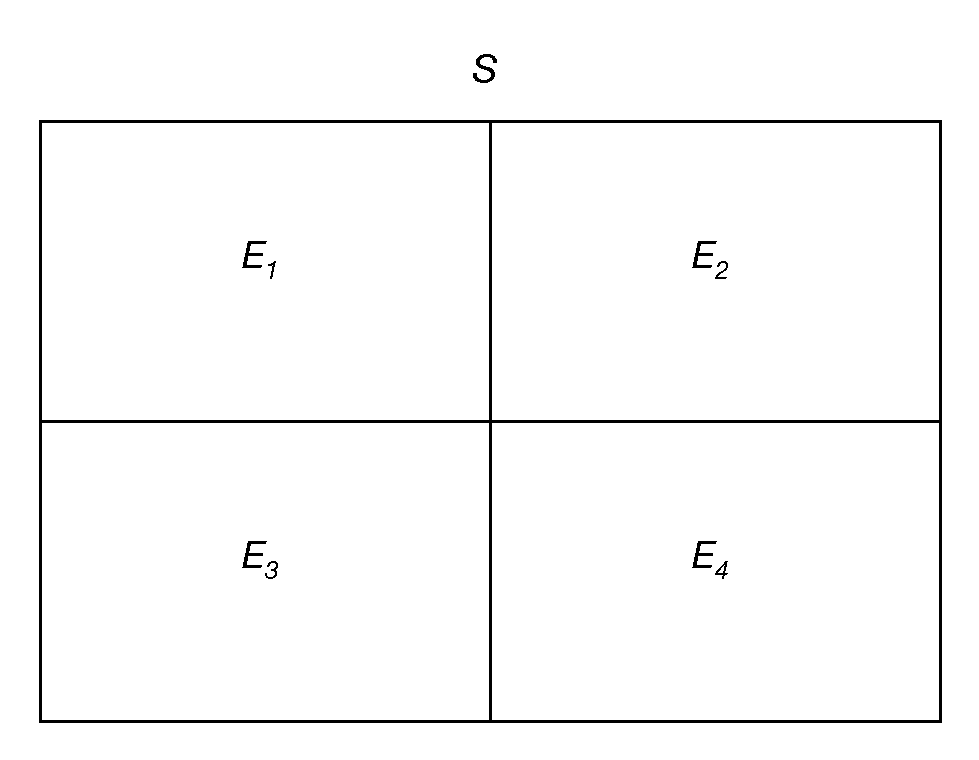
\includegraphics[width=5cm]{partition.eps}
\end{figure}

If $A$ is any event, and $\{E_1, E_2, \dots, E_k\}$ is a partition of $\cals$, then we can decompose $A$ according to the partition by:
\[
A = (A \cap E_1) \cup (A \cap E_2) \cup \cdots \cup (A \cap E_k)
\]
where this union consists of disjoint sets (since the partition consists of disjoint sets). For $k = 4$, this is illustrated graphically below:
\begin{figure}[H]
\centering
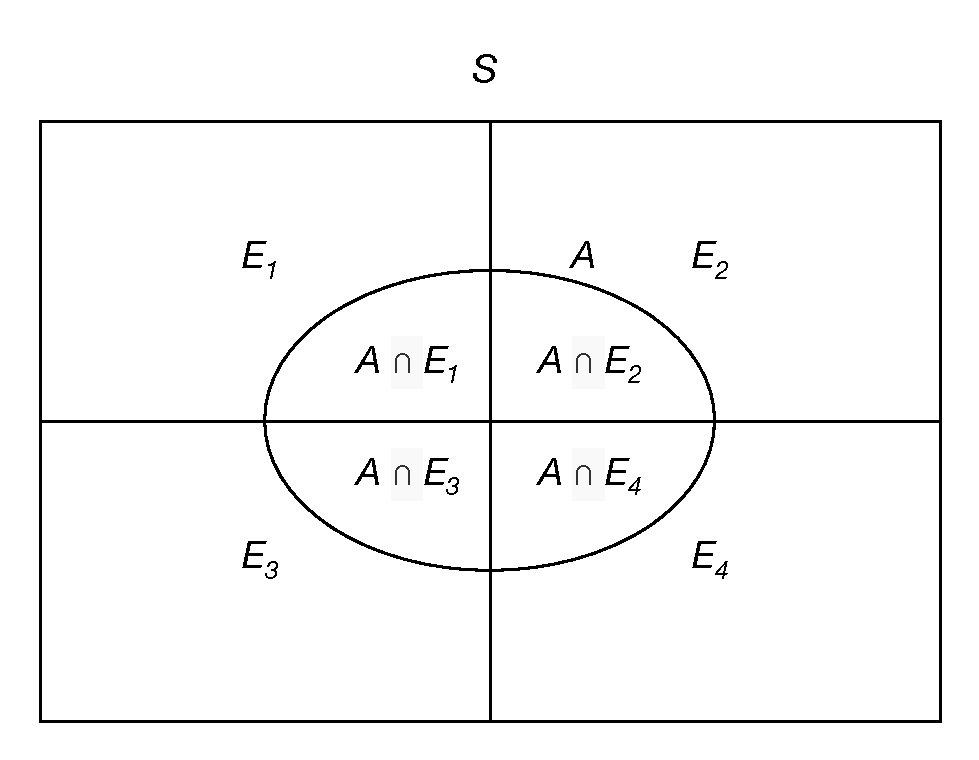
\includegraphics[width=5cm]{partition2.eps}
\end{figure}

We are now ready to state the Law of Total Probability.

\begin{framed}
\emph{Law of total probabiltiy}\\
  \rule{\dimexpr\linewidth-2\fboxsep-2\fboxrule}{.1pt} \\
Let $\{E_1, E_2, \dots, E_k\}$ be a partition of $\cals$ such that $\P(E_i) > 0$ for all $i$. Then for any event $A$, we can decompose the probabiliy of $A$ according to our partition as:
\[
\P(A) = \sum_{i = 1}^k \P(A|E_i)\P(E_i)
\]
\end{framed}
To see this is true, first we decompose our event $A$ as we did above into disjoint sets:
\[
A = (A \cap E_1) \cup (A \cap E_2) \cup \cdots \cup (A \cap E_k)
\]
Then we can write:
\begin{align*}
\P(A) &= \P( (A \cap E_1) \cup (A \cap E_2) \cup \cdots \cup (A \cap E_k) ) \\
&= \P(A \cap E_1) + \P(A \cap E_2) + \dots + \P(A \cap E_k) \\
&= \P(A|E_1)\P(E_1) + \P(A|E_2)\P(E_2) + \dots + \P(A|E_k)\P(E_k) 
\end{align*}
where we have used the fact that the decomposition of $A$ is a union of disjoint sets, and have also used the definition of conditional probabilility.\\

We can now combine Bayes' rule and the Law of Total Probability to get another version of Bayes' rule.

\begin{framed}
\emph{Bayes' rule, total probability version}\\
  \rule{\dimexpr\linewidth-2\fboxsep-2\fboxrule}{.1pt} \\
Let $A$ and $B$ be two events, and let $\{E_1, E_2, \dots, E_k\}$ be a partition of $\cals$ such that $\P(E_i) > 0$ for all $i$. Then:
\begin{align*}
\P(A | B) &= \frac{ \P(B|A)\P(A)}{\sum_{i=1}^k \P(B|E_i)\P(E_i)}
\end{align*}
where $\P(B) \neq 0.$
\end{framed}
To get this, take Bayes' rule and expand $\P(B)$ in the denominator using our partition and the Law of Total Probability.\\

Let's revisit the drawing-balls-from-bags example one final time, using the total probability version of Bayes' rule.

\begin{example}You have two bags of balls. The first bag contains one red ball and three white balls. The second bag contains two red balls and two white balls. You choose a bag uniformly at random and then draw a ball from the chosen bag. What is the probability that you choose the Bag 1 in the first step given that the ball drawn is red?\\

Using the same events as in the above two versions, we are once again looking for conditional probabiltiy $\P(B_1|R)$. Our partition is $\{B_1, B_2\}$ since one of these two events must occur (so the union is $\cals$), but both cannot occur (so they are disjoint). Writing out Bayes' rule, we get:
\[
\P(B_1|R) = \frac{ \P(R|B_1)\P(B_1)}{ \P(R|B_1)\P(B_1) + \P(R|B_2)\P(B_2) }
\]
The probabilities involved in this are straightforward:
\begin{enumerate}
\item $\P(B_1) = \P(B_2) = 1/2$
\item $\P(R|B_1) = 1/4$
\item $\P(R|B_2) = 1/2$
\end{enumerate}
So we just plug these in to get:
\[
\P(B_1|R) = \frac{ (1/4)(1/2)}{(1/4)(1/2) + (1/2)(1/2) } = \frac{1/8}{3/8} = \frac{1}{3}
\]
which agrees with both versions above!
\end{example}

\begin{example}Consider the following card game. We have 3 cards that are identical in shape and size. The cards are colored as follows:
\begin{enumerate}
\item both sides are red
\item both sides are black
\item one side is red and the other side is black
\end{enumerate}
The three cards are shuffled and one is randomly chosen and it put down on a table. If the face-up side of the chosen card is red, what is the probability that the other side is black?\\

Let $RR$, $BB$, and $RB$ denote the events that the chosen card is all red, all black, or red-black (respectively). Let $R$ be the event that the face-up side of the chosen card is red. Note that $\{RR, BB, RB\}$ is a partition of our sample space. We are interested in whether the red-black card has been chosen, i.e. $\P(RB|R)$. First we write out the total probability version of Bayes' rule, then we plug in the probabilties we know:
\begin{align*}
\P(RB|R) &= \frac{ \P(R|RB) \P(RB) }{ \P(R|RR)\P(RR) + \P(R|BB)\P(BB) + \P(R|RB)\P(RB) } \\
&= \frac{(1/2)(1/3)}{ (1)(1/3) + 0(1/3) + (1/2)(1/3) } \\
&= \frac{1/6}{1/2} \\
&= \frac{1}{3}
\end{align*}
Thus the probability that the other side is black is only 1/3. It is tempting to guess that that the probability of the other side being black is 1/2 since there are two possible cards it could be (all red and red-black), and they should be equally likely. It turns out that this is not the case! The two cards are not equally likely. Here is one way to see this. Instead of considering three cards, let's think of them as six sides. We can label the six sides as:
\begin{enumerate}
\item $R_1$ and $R_2$: the two red sides of the all-red card
\item $B_1$ and $B_2$: the two black sides of the all-black card
\item $R_3$ and $B_3$: the red and black sides of the red-black card
\end{enumerate}
If red is face up, it must be $R_1, R_2$, or $R_3$, and these are equally likely. For $R_1$ and $R_2$, the other side of the card is red. Only for $R_3$ is the other side black. Thus the probability of the other side of the card being black is 1/3, which agrees with the result from Bayes' theorem.
\end{example}

Here is another application of Bayes' theorem which concerns medical testing. This is a classic example in the field of public health.

\begin{example}
The OraQuick HIV test is a rapid test for HIV, which can give a result in 20 minutes. The test has the following properties:
\begin{enumerate}
\item Sensitivity (probability of a positive test given that you have the disease): 0.996 (99.6\%)
\item Specificitiy (probability of a negative test given that you don't have the disease): 0.999 (99.9\%)
\end{enumerate}
What is the positive predictive value of the test, i.e. the probability that a patient has HIV given that the OraQuick test is positive\footnote{Sensitivity, specificity, and positive predictive value are public health terms; you don't have to know them. Data here is from the CDC website.}.\\

Let $T$ be the event that the test is positive, and $H$ the event that the patient has HIV. We are interested in the positive predictive value, which is $\P(H|T)$. Let's write out Bayes' rule:
\[
\P(H|T) = \frac{ \P(T|H)\P(H)}{ \P(T) }
\]
We cannot possibly know the denominator $\P(T)$ (the probability of a positive test), so we will use the total probability of Bayes' theorem, with partition $\{H, H^c\}$.

\[
\P(H|T) = \frac{ \P(T|H)\P(H)}{ \P(T|H)\P(H) + \P(T|H^c)\P(H^c) }
\]
What do we know? $\P(T|H)$ is the sensitivity, so that is 0.996. We don't know $\P(T|H^c)$, but we do know the specificity, which is $\P(T^c|H^c) = 0.999$. Since $\P(T|H^c) + \P(T^c|H^c) = 1$ (either the test is positive or it's not), $\P(T|H^c) = 1 - \P(T^c|H^c) = 1 - 0.999 = 0.001$. All that remains is $\P(H)$. ($\P(H^c) = 1 - \P(H)$, so we are all set once we have $\P(H)$.) What is $\P(H)$? That is the probability that a randomly-selected patient has HIV, what is known in public health parlance and the disease prevalence. This can be a hard quantity to determine and is the crux of this entire problem.\\

The CDC estimates that 1.2 million people in the US have HIV\footnote{This estimate is for the end of 2012, but is the most recent CDC data I can find.}, out of a total population of 319 million. That puts the prevalence of HIV at 0.00376. So we will take $\P(H) = 0.00376$ for now, which gives us $\P(H^c) = 1 - 0.00376$. Plugging everything into Bayes' theorem:
\[
\P(H|T) = \frac{ (0.996)(0.00376)}{ (0.996)(0.00376) + (0.001)(1 - 0.00376) } = 0.79
\] 
So we get a positive test in 80\% of the cases, which is decent but not great. Let's repeat this with a different value for the prevalence of HIV. In Fulton County, GA (which contains Atlanta) the prevalence of HIV is approximately 0.0123 (significantly higher than for the nation as a whole). This gives us a positive predictive value of:
\[
\P(H|T) = \frac{ (0.996)(0.0123)}{ (0.996)(0.0123) + (0.001)(1 - 0.0123) } = 0.925
\]
which is higher. The take-home message here for public health is the following. The positive predictive value of a  test depends on the prevalence of the disease you are testing for; it increases as a disease becomes more common, i.e. increases with disease prevalence. Even the most sensitive and specific test does a poor job of detecting rare diseases.
\end{example}

\end{document}
